\documentclass[11pt]{article}

\usepackage[margin=1in]{geometry}
\usepackage{amsmath, amssymb, amsthm, mathtools}
\usepackage{fancyhdr}
\usepackage{hyperref}
\usepackage{tikz}
\usepackage{graphicx}
% \begin{figure}[htbp] % [htbp] 告诉 LaTeX 尽量放在这里、顶部、底部或单独一页
%     \centering % 图片居中
%     \includegraphics[width=0.5\linewidth]{filename} 
%     \caption{这是 MATH154 HW1 的图示} % 图片下方的标题
%     \label{fig:graph1} % 用于文中引用，比如 "如图 \ref{fig:graph1} 所示"
% \end{figure}

\setlength{\parindent}{0pt}
\setlength{\parskip}{0.5em}

\newcommand{\R}{\mathbb{R}}
\newcommand{\N}{\mathbb{N}}
\newcommand{\Z}{\mathbb{Z}}
\newcommand{\Q}{\mathbb{Q}}
\newcommand{\C}{\mathbb{C}}

\newenvironment{problem}[1]
  {\section*{Problem #1}}
  {}



\begin{document}

\title{Homework 5}
\author{Jamie Meng}
\date{\today}

\maketitle
\section{Problem 1}
\subsection*{(a)}
A matching of G is the following:

Connect 1 with a, Connect 2 with d, Connect 3 with b, Connect 4 with c.
No maching exist in H, because the set $\{1,2,4\}$'s neighbor set is $\{b,c\}$, which has a smaller size. Therefore, according to Hall's theorem, no such matching exits in H.

\subsection*{(b)}

\begin{figure}[htbp] % [htbp] 告诉 LaTeX 尽量放在这里、顶部、底部或单独一页
    \centering % 图片居中
    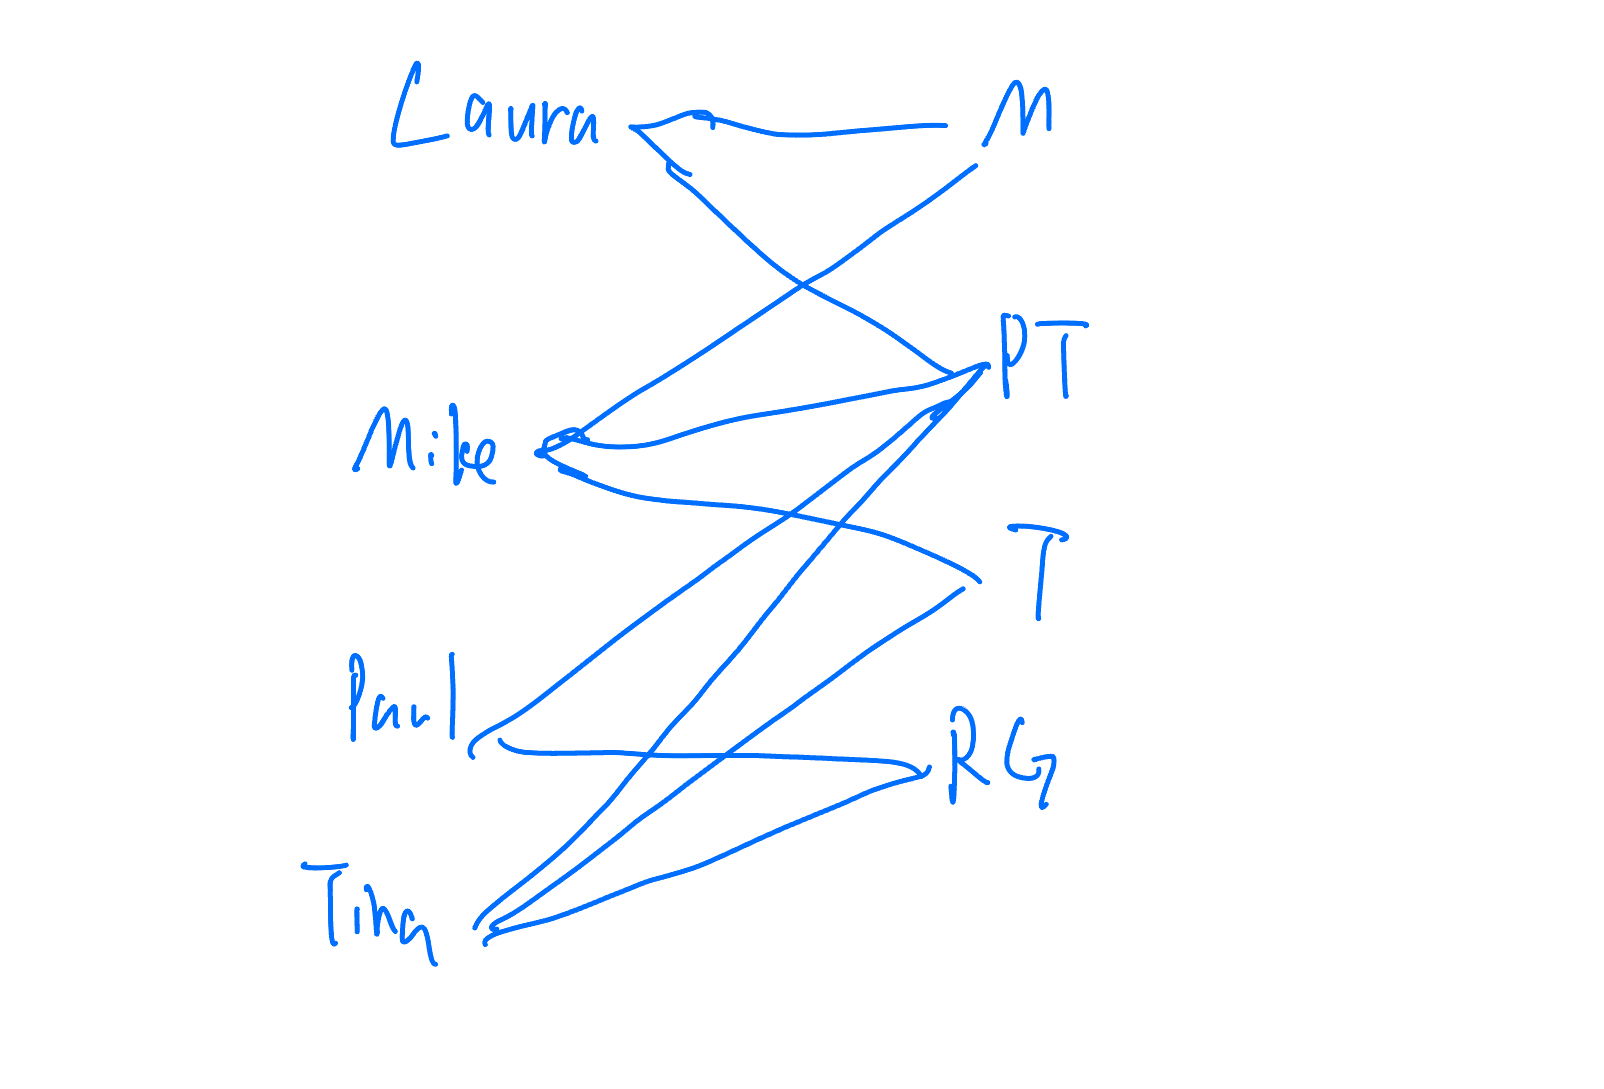
\includegraphics[width=0.5\linewidth]{NBMetadataCache.jpeg} 
    \label{fig:graph1} % 用于文中引用，比如 "如图 \ref{fig:graph1} 所示"
\end{figure}

There exist a matching:

Laura-M

Mike-PT

Paul-RG 

Tina-T 

Therefore, Hall's condition must be satisfied according to Hall's theorem. 
And a assignment can be:

Laura-M

Mike-PT

Paul-RG 

Tina-T 
\subsection*{(c)}
This problem can transition to a matching problem. The set A is the professors set, and set B is the committees set. Each professor's vertex has 3 neighbors. And each committees set has 6 neighbors. We need to prove there exists a matching covering set B.

We can use hall's theorem to verify it. Suppose the set S has n vertices. Then, the total degree is 6n. Then, N(S) has at least 6n degrees in total. Beucause each professor only has 3 neighbors, there must exist 2n professors. Because 2n is greater than or equals to n, hall's condition is verified, and there exists a matching covering set B, and we are done.

\section{Problem 2}
\subsection*{(a)}
Lemma: any k-regular bipartite graph contains a perfect matching:

Since it is a K-regular bipartite graph we can divide the vertices in to set A and B base on their color. Therefore, the total degree in A is $K * |A|$ which equals to the total degree in B, which is $K * |B|$. Therefore, |A|=|B|. For any sets S in A, the total degree is $K * |S|$. Therefore, the total degree of N(S) must be greater than or equals to $K * |S|$. Then, the total number of vertices is  greater than or equals to $|S|$. Then, hall's condition is satisfied. The lemma is proven.

Back to the problem. Since it is a k-regular graph, it has a perfect matching. Then we can delete all edges in the matching to form a edge set. And the graph become a k-1-regular graph, and it also has a perfect matching. We can repeat this process for k times. Then, we got k edge sets. They are disjoint and are perfect matching. Therefore, its edge set E can be written as the union of k edge-disjoint perfect matchings.

\subsection*{(b)}

The total degree in A and B is same. Therefore, $$|A|a=|B|b$$
Since, $$|A|\le|B|$$
Therefore, $$a\ge b$$

For any edge set S in A. The total degree is $|S| a $. And the total degree of its neighbor set must greater than or equals to its total degree. Therefore, 
$$|N(S)|b \ge |S|a $$
Since,$$a\ge b$$ Then
$$|N(S)| \ge |S| $$
And Hall's contition is satisfied, then there exists a matching covering A. Then, G contains a matching of size |A|.

\section{Problem 3}
\subsection*{(a)}
We can pick any edge between A and B. And let be a part of a matching. Since the end points of the edge is matched, we can delete them and all edge connnecting them. For the rest of the set, any non-empty set X in A(without the deleted vertex), $|N(X)| > |X|$ before the deleting. If the deleted vertex in B is in N(X), then new |N(X)| will decrease 1, so $|N(X)| \ge |X|$ And hall's condition is meet. Therefore, there exists a matching covering rest of A. Add back the deleted matching.  We found a matching covering A with one specific edge to include. Therefore, every edge of G belongs to some matching M that covers A.

\subsection*{(b)}
We can first prove that there exists a matching of size$|A| - d_*$, we can add $d_* $ additional vertices to set B, and let them connect to all vertives in A. Then N(S) increases $d_*$ for all S. Since $d_*$ is the maximum difference of N(S) and S, then hall's condition is satisfied. Therefore, A has a matching covering A with B+ $d_*$ additional vertices. Then we can delete these $d_*$ additional vertices, and the matching size will decrease at most $d_*$. Then, there still exists a matching of size$|A| - d_*$.

Then, we can prove why this is the maximum. 

Because there exist a set S that $|S| - |N_G(S)| = d^*$. In original graph. The set S can only match vertices in $N_G(S)$. Therefore, $d^*$ vertices cannot be matched. Since only in set S $d^*$ vertices cannot be matched, in set A, greater than or equal to $d^*$ vertices cannot be matched.

Therefore, he maximum matching of G has size $|A| - d_*$.

\subsection*{(c)}

Given a set $S \in A$ that violates Halls condition, consider the set of vertices H in B not adjacent to S. All H in won't have neighbor in set S. 

Because $$|S|> |N(S)|$$
Then because $|A|=|B|$
$$|A/S| < |B/N(S)|=|H|$$
And because $$|N(H)|\le |A/S| $$
Therefore, $$|N(H)|< |H| $$
Then, H also violates Halls condition. And we are done.


\end{document}
